\chapter{Introduction}

%1st paragraph/section: context summary: why
\section{context summary, why, and motivation}
%Topic in a sentence: knowledge retention including into a system. The system does machine learning on extreme-scale data

One of the main paradigm shifts currently ongoing within machine learning is developing models that can handle evolving tasks and environments. While the literature on algorithms able to retain knowledge is increasing, systems approaches to this problem are lagging behind, and systems presented in literature systematically lack reasoning on why the design decisions presented were made.

To contribute to filling this gap, an inspection of systems approaches for enabling long model lifetimes within the context of maritime is conducted. The case in question is highly geographically distributed, voluminous in data, and does not require instant response times. The aim is to thoroughly compare and assess approaches for dealing with evolving model environments and discuss which approaches suit the case and its set of requirements. Then, it is discussed what kind of big data system design would optimally enable implementing the knowledge retention approach chosen.

In addition to presenting a system proposal for the specific case, as a conclusion is also discussed, which requirements led to which design decisions to elaborate how the insights derived in this case can be transferred to another case.

The way in which this work differs form many other system presentations is that the goal is not only to find a solution that works, but to find a solution that has the highest chance of succeeding in operation. This means that some less technical considerations are also included. These are simplicity and maturity of the solution, as these traits arguably increase the chance that a system working in theory actually works in practice.

% outline: topic, backgound summary, motivation

% things to mention:
% the paradigm shift
% lack of systems literature addressing whys
% maritime requirements
% the intention: find vesselai optimal solutions
% further intention: find applicability to other cases
% take into account: maturity, simplicity. Not only find a system that works but the one that has the highest probability of succeeding in operation

% to-adds: that maturity is a factor that ended up being the very one reason many promising-seeming approaches cannot be adopted in this case


%2nd paragraph/section: question, results, methodology
\section{research questions, results summary and methodology}

primary question: Which model adaptation approach would be optimal for maintaining model accuracy across a long lifetime in the specific context of vesselai?

ssecondary question, option #1: what kind of workflow automation needs to be in place in order to have the models updated as efficiently as possible

secondary question, option #2: what type of infrastructure is needed to facilitate the chosen approach for model lifetime extension in the system?

%outdated
a point of motivation from D1.1 moving beyond the state of the art section: ''the time is ripe  to  rethink  whether  cloud  computing  is  the  only  architecture  able  to  support  IoT  applications, especially  in  the  case  of  smart applications,  where  static  and  mobile  IoT  devices  will  be  widely embedded  in  infrastructures.  It  is  worth  investigating  an  overall  orchestration  of  the  computational resources  available  today  that  can  take  advantage  of  the  edge-fog-cloud  continuum'' addition: to make lifelong learning possible

methology

when comparing systems, only systems handing spatiotemporal data are considered

when comparing model updating approaches, classifie



results summary

\section{Chapter roles}

% this should maybe be shortened? in many papers this section is much shorter and only outlines the highest level, ie here chapters maybe

The rest of this thesis is organized as follows:

Chapter 2 presents the necessary background knowledge to the reader. First, a general introduction into distributed big data systems with machine learning is given. The high-level components, such as data preprocessing and model training, are presented. Then, some general best practices for big data systems design are discussed.

A more thorough state-of-the-art inspection is given in the domain of machine learning on the methods for extending the lifetime of a model. The main challenges in this, the concept drift and the stability-plasticity-dilemma are defined, and then the existing solutions for addressing the challenges are presented.

Next, the general context for the VesselAI project is described. The specialities of the maritime domain and the nature of the data sources are dissected, after which the project pilots and general goals are presented. From these the general requirements are listed and the main challenge of the project is identified: how to organize a workflow for efficient adaptation of the models.

Chapter 3 analyzes and compares the various model updating approaches presented previously while taking into great consideration the point of view of the case studied. The implications of this to the machine learning workflow and the required infrastructure are inspected for optimal trade-offs. After this, the VesselAI system proposal is presented, alongside reasoning why these decision should be made. It is also considered whether there is enough evidence to make the presented conclusions, or if there are several good-seeming options to choose from.

The paper is concluded with discussion on if the conclusions reached with the case study are applicable to other systems with similar requirements. Especially applicability to other cases with highly voluminous data combined with a long model lifetime is emphasized.

\chapter{Context and Background}

\section{On Big Data Systems With Machine Learning}

% MLOps is a term that should be used / mentioned somewhere

% current main concern for this sect: I state out a lot of facts without giving a reference -> the fine line between common knowledge and what needs backing...

\subsection{The high-level components}

% is this section necessary?

The steps that most large-scale machine learning systems compose of are displayed in the following figure: 

% how do I properly cite the google cloud developer guide?
% the figure is too small... -> not very readable
\begin{figure}[ht]
%\begin{figure}[tbh] t= top, b = bottom, h=here
\ \newline
\begin{center}
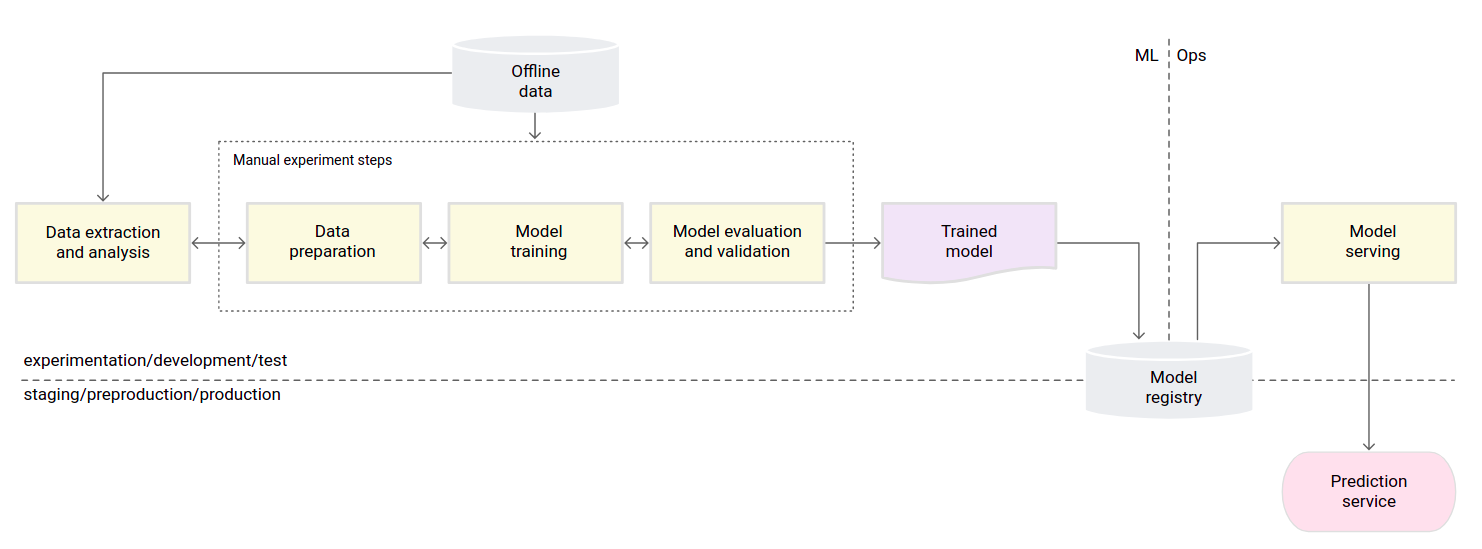
\includegraphics[width=0.9\textwidth]{simplegoogle.png}
\caption{Abstract components of a big data analytics system. From Google Developer MLOps guide \cite{googlemlops}.}
\label{simplepipeline}
\end{center}
\end{figure}


While the steps above represent a coarse abstraction, hiding away feedback loops and the multitudes of ways each part can be implemented, most contemporary big data systems implement all of the following steps:

\textbf{Data extraction}: this component is responsible for handling the incoming data. Usual forms of data are either web logs, coming in from a server, or IoT data, coming in from sensors that are often geographically distant from the data ingesting component.
% that data is usually web logs or sensor requires a reference?

In big data systems incoming data is represented either as batches, meaning chunks of data coming in at certain intervals, or as a stream, meaning that individual data records are coming in constantly. The main advantage of using a batch representation is known to be increased throughput%(find citations here)
, while stream processing allows smaller end-to-end latencies. %(find citations here)
% the usually interpreted as stream or batch needs a ref too?

To mitigate the tradeoff between throughput and latency, a popular solution is called the lambda architecture. This reference architecture has a processing unit for both batch and stream data with the stream component, so-called speed layer, handling requests for the data not yet processed by the batch layer \cite{beatingcap}. While this approach is widely accepted to solve the problem of handling highly voluminous data fast and mitigating human errors by allowing restarting the speed layer any time without losing data \cite{lambdakappa}, the architecture has faced criticism for being redundantly complex and forcing the data ingestion code to be written twice \cite{questioninglambda} \cite{uber} \cite{facebook}. As an alternative, the kappa architecture has been proposed, only composing of either a batch or a stream processor, usually the latter \cite{questioninglambda}. This mitigates duplication, but retains the tradeoff with throughput and latency \cite{lambdakappa}.

\textbf{Data preparation}: This step encompasses the processes of data cleaning, transformation, and feature engineering. Data cleaning refers to operations identifying and removing faulty data, such as values that are missing or are clearly impossible. Data transformation and feature engineering are used interchangeably, both meaning processes that transform data into a format that the models used can process. A popular example in this is the mapping of plain text into word count matrices \cite{dapbook}.

While the data preparation step is often overlooked in literature,
it is a both challenging and crucial part of the system as preprocessing commonly takes up a majority of the total end-to-end latency of a machine learning system \cite{adaptivelearningsystems}. As for systems design, the most relevant decision to make is whether to clean data before it is saved to the data storage, or only when it is  needed for training. The main benefit with the first approach is that data only needs to be cleaned once, while the latter allows processing data for different models in different ways.
% the two approaches and their tradeoffs need a ref...
% the how many % of time preprocessing takes needs a ref... i got one somewhere...

\textbf{Data storage}: Interpreted in the figure as offline data, the data storage is used to save the data that is needed for model training. The most often used storage methods are called data warehouses and columnar databases. Due to the volume of the data, the storage is either cleared often completely or only a small part of the data is archived.
% data archival needs a ref.
% popular ways of implementing data storage too!

\textbf{Model training}: This component is responsible for training the model, which means tuning the model parameters in a way that it fits to the distribution of the incoming data in order to make accurate predictions from data coming in during operation.

The training conducted can be done from scratch, meaning that the same instance of the model has not been trained before, or in cases of using adaptation-capable models, the models can be updated. Details on model updating or retraining are discussed below.

As for infrastructure, training can be conducted in a central or federated manner. Centralized training, often run in a cloud data center, can run either on one machine or distributed across multiple cores by splitting the model or the data to parallelize the training \cite{iotsurvey}. As the amount of data is large, high-performance computing (HPC) clusters and modern general processing units (GPU) are used to reach required latencies \cite{iotsurvey}. Federated approach refers to an internet of things setting where the training is conducted in the edge devices of the IoT network. This aims to solve the issues of moving privacy-sensitive data across the network and being able to adapt to the unique environments of each data source \cite{iotsurvey}. As in the maritime context the data is neither highly private or has differing environments in different sensors, the federated approach is not considered further in this work.

\textbf{Model evaluation and validation}: In this stage the model is tested and adjusted in various ways. For testing, usually various model metrics such as accuracy for classifiers and error statistics for regression tasks are checked \cite{iotsurvey}. These numbers can also be compared against other models, possibly models already in operation \cite{googlemlops}. Also testing different data sets and checking compatibility with the rest of the system is conducted at this stage \cite{googlemlops}.

In addition to testing, models are also optimized for the infrastructure that they are being deployed on. This can include, for example, various performance optimizations, or in case of constrained memory, model compression \cite{iotsurvey}.

\textbf{Model registry}: is a centralized storage for the trained models. 

% need a reference here as well...

\textbf{Model inference}: edge fog cloud here marked in the figure as 'prediction service', this component contains the trained models that are used for answering application requests. These requests can require data statistics, computed with conventional data analytics, or predictions made by machine learning models.

The most important design decision to make for this component in the sensor data scenario is where to deploy the models, in the cloud, a cloudlet or 'fog', or on the edge. Cloud means that the model is deployed in a data center and edge refers to models being deployed in the IoT devices. Fog refers to the in-between solutions: 

OCF is The Open Connectivity Foundation. add below + the proper source

The definition of fog computing is the following, as stated by the the OCF (in \cite{fogsurvey} reference [42]): “Fog computing is a horizontal, system-level architecture that distributes computing, storage, control and networking functions closer to the users along a cloud-to-thing continuum.” (but not only entirely to the edge). Or, put differently by \cite{fogsurvey} for a clearer mental image: "The Fog is a Cloud closer to the ground."

\subsection{Best-practice design principles}

%\cite{designprinciples}: most important things are system stability with fluctuating data quality, scalability, minimal human intervention

%\cite{facebook}: ease of use, performance, fault-tolerance, scalability, correctness

%\cite{storm@twitter}: scalable, resilient, extensible, efficient, easy to administer

%\cite{uber} always a tradeoff between requirements, quick iteration for improvements, quich scaling in hardware

%\cite{millwheel}: fault tolerance, scalability

%--> synthesized there is scalability, resiliency for faults & environment changes, easy to improve the system 

%also some genaral principles on bd systems. Tradeoffs is big: usually to achieve better results in some respect simplicity is sacrificed. The goal is to do complex in right places where real benefits can be received, and keep it simple elsewhere. Also point on this is that the big mature big data systems stated that simplicity or ease of use or maintainability, basically variants of simplicity, is the most imporant trait or one of the most important

In order to design a working big data system, taking into account lessons and best practices learned in the past greatly increases the chances of succeeding in operation. In general, as stated by the authors of \cite{uber}, in systems design everything is a tradeoff: every design decision taken to improve the system in some respect inevitably will degrade quality in another respect. At its simplest, for instance, improving the systems throughput by adding ... (what?) in a way adds complexity, meanwhile sacrificing simplicity.

The most mature big data systems as of date have each evolved on their own but despite that have identified quite similar best practices, that should be preferred no matter the field of implementation. In each system compared, Google MillWheel \cite{millwheel}, Facebook \cite{facebook}, Twitter storm \cite{storm@twitter}, the M6D ad targeting engine \cite{designprinciples}, and the Uber system \cite{uber}, there is a slight variance in emphasis of importance and naming of each one, but in general the following traits were deemed the most important across all systems:

\begin{itemize}
    \item \textbf{Ease of using and improving}: while others named this as 'ease of use', others named 'easy to administer', 'easy to improve' or 'minimal human intervention', in general all terms refer to how usable the system is. Its operation should be effortless, but at the same time, improving it should be quick, as this enables fast adaptation to ever-changing application needs. In addition, modularity is in this respect important as it enables iterating individual modules, and simplicity in general makes a system both usable, and easier to update.
    \item \textbf{Scalability}: Scalability was named as one of the most important trait to favor across all systems descriptions listed. Scale is at the core of the nature of big data, and with expectations of the amount of data doubling every x years (need a reference for this), it is reasonable to constantly be prepared to handle ever-growing quantities of data. This can be achieved through various solutions of distributed computation, or making adding more hardware to the system as seamless as possible.
    \item \textbf{Resiliency}: Under this umbrella term fit both the terms fault tolerance and resiliency to changes in the operational environment. With big systems consisting of multitudes of components and different types of infrastucture, individual parts of the system failing is a very common occurence. In addition, in terms of the machine learning conducted in the systems, the models should be able to perform in a stable manner, meaning that the prediction accuracy variance should stay small despite minor changes in the incoming data, or other changes in the environment.
\end{itemize}

\section{Model adaptation techniques for machine learning}

% to-do: add adaptive learning approaches to the first subsect and remove subsectioning

\subsection{Definitions}

% this section: I should have more sources and double-check that I got the definitions correct.

% mention the types of adaptive learning earlier

% find reference to "There are two broad ways of retaining knowledge"

% Knowledge retention is a self-invented term and should be replaced with a better one.

% online learning is kind of synonymous to stream processing and can (?) be taken as given. define it here or elsewhere, in systems possibly.

In machine learning based systems, the term \textbf{knowledge retention} means extending the span of time of a machine learning model from months to years while preserving its performance. Here ''knowledge'' means the model parameters that resulted from training a machine learning model of a specific machine learning task. There are two broad ways of retaining knowledge. Firstly, one can use a model for a specific task in an environment that is shifting over time. This is called \textbf{adaptive learning} \cite{conceptdriftsurvey}. Secondly, a model can be used in multiple tasks; the knowledge gained from training for one task can be transferred to similar problem domains. This is referred to with \textbf{transfer learning} \cite{lmlsystems}.

The paper at hand is dealing with the problem of adaptive learning. However, as terms can be easily confused and misunderstood, some terms regarding transfer learning are defined next.

\textbf{Lifelong learning} is a machine learning paradigm of ''learning many tasks over a lifetime from one or more domains'' \cite{lmlsystems}. This means that the knowledge gained from one task is processed in a way that it can be applied to a related task. As of date lifelong learning is implemented for simple classification tasks, and the new tasks are usually introduced by including unseen classes of data for the testing data set \cite{lmlinneuralnets}. A new environment could also perhaps be interpreted as a new task, but as the paradigm is currently still new and tackling very simple problems \cite{lmlinneuralnets}, it is too early for its adoption to a real-world scenario with complex models.
% stability-plasticity is a transfer learning problem. omit.
The general challenges arising in knowledge retention are the following. Especially within transfer learning \textbf{the stability-plasticity dilemma} is central. This refers to the need of finding an optimal balance on when to retain the old knowledge (stability) and when to replace it with new insight (plasticity) in order to perform well in predicting for both the old tasks seen and the new ones emerging later. Overdoing plasticity, i. e. replacing old parameters too easily may sometimes lead to \textbf{catastrophic forgetting}, which means that the ability to predict accurately for the old tasks is lost completely or for a big part.

% add: that the only legitimate option to drift mitigation is retraining, which is cpu-heavy.
Within adaptive learning the central problem to address is called \textbf{concept drift}. This means, in technical terms, that ''the relation between the input data and the target variable changes over time'' \cite{conceptdriftsurvey}. This is usually the result of changes in the environment in which learning is conducted. For example, in the maritime domain, it is possible that over the years vessels' speeds increase, and as a result the old trajectory forecaster predicts systematically false future locations for vessels.

The concept drift can include in itself a need for balancing stability and plasticity, depending on the use case. In autonomous cars, for example, an adaptive learning algorithm could change its predictions based on shifts in lighting and terrain conditions, but it should still be able to operate in the conditions it has seen before the changes \cite{conceptdriftsurvey}. In contrast, in maritime, it is not necessary for the models to perform well in an environment of the past after marine traffic conditions have shifted over time.

% maybe add here the definition of feature drift: "A feature drift occurs when a subset of features becomes, or ceases to be, relevant to the learning task [10]" (from mlflorstreamingsurvey) -> feature evolution will be a rare occurence in vesselai, can be omitted? also streamminingchallenges stated that feature drift is an important problem to address!

% maybe add: also hyperparams need to evolve! \cite{mlflorstreamingsurvey}

% maybe add: there is gradual and abrupt drift \cite{streamminingchallenges} \cite{conceptdriftsurvey}

\subsection{Implementing adaptive learning}

In the following section the ways of mitigating the effects of concept drift whilst maintaining performance on old tasks, if necessary, are presented.

The ways of doing adaptive: retraining, incremental learning, online learning. Then there was the ways of preserving old data and re-feeding it to models. Then there are the ensemble learning techniques, putting models to sleep state, blind&informed adaptation, ways for feedback mechanisms
% ! zliobailte's concept drift survey (not conceptdriftsurvey but the 2nd): incremental learning is not related to adaptation, it is a different domain! do not confuseeeee
-> there are a lot of ways, many ways to classify the ways also. Make more sense of what each means and how they should be presented. Find more sources than \cite{conceptdriftsurvey} to find more insight.

definitions
 retraining: taking a new instance of the model and completely training it again from scratch
	    incremental learning: a model is trained with each batch coming in from a data source and updated after each training. a way of doing adaptive learning.
	    online learning: the model is updated with each data entry coming in from a data stream and is simultaneously constantly in operation. a way of doing adaptive learning.
	    ensemble learning: adapting through predicting with a combination of models

% add here: in order to implement adaptive learning, a few new components need to be introduced. Then display the more complex system description and explain with emphasis the trigger and monitoring

% iotsurvey has a decent seeming sect on the monitoring stuff

\section{The case: context and requirements for machine learning in the maritime domain}

Maritime as a domain of application for a sensor-based machine learning system is in a few ways significantly different from many others. The most obvious difference is its global nature; domains like smart cities also have to take into account the fact that there is some geographical distribution, but with the seas covering x\% of the earths' surface, the extent of geographical distribution in the maritime context is on a whole new level.

With the vastness of the seas and its vital nature for world trade, the amount of vessel traffic is large even in comparison to other big data applications. Due to international regulation vessels have to send update signals on their status from every few minutes to every 2 seconds, depending on their speed and course \cite{maritimeinformatics}. With approximately 100, 000 ships sailing the world oceans daily (a source from \cite{maritimeinformatics} states this), this leads to several billion messages sent each day. To this exceptional amount of data we refer to as \textit{extreme-scale data} in this work. In addition to this, in order to provide valid maritime intelligence, other types of data such as geographical information and weather updates, are needed. Therefore, the data is not only highly voluminous, but also heterogeneous, coming in both static and dynamic forms at different velocities.

Added to scale, another specific of this context is speed. Depending on the size and type of the vessel, it takes from minutes to up to an hour to change the course of the vessel (todo: fact-check this). This means that for the AI services targeted for navigational purposes the end-to-end latencies need not to be faster than the order of minutes, and execution times of up to 30-60 minutes can be acceptable. For other AI services end-to-end times in order of seconds may be aimed for, but achieving sub-second latencies as is often the goal in literature (citations...), is unnecessary, even of detriment to the success of the system operation: for low latency other more important traits would have to be deprioritised, which in this case would do more harm than good.

The main data source, the status signal data sent by vessels, called \textit{automatic identification system} (AIS) data, also has its specialities. AIS is a form of sensor data and has two types: static messages containing information such as name, destination and ship characteristics, and dynamic messages with information on the vessels' location, speed, heading, and rate of turn. The challenge with AIS data is both its highly fluctuating reporting intervals and especially its unreliability.  Things such as manually written destinations, faulty timestamping, lack of universal identifiers, unreceived sensor messages, misreported locations, and even illegal traffic camouflaging their operations, make identifying and correcting erroneous data both difficult and computationally intensive.

The goal on the application level of the VesselAI project is to provide the following four pilot services to users: vessel route forecasting for traffic monitoring and management, design of optimal ship energy systems, operating autonomous ships in short sea transport, and weather-optimized routing for long-distance voyages. More abstract goals are to find a system that is suitable for both managing extreme-scale data and facilitating long model lifetimes. The goal is also to be able to fully utilize the most modern high performance computing infrastructures in an optimal way.

With this context specification in mind, the following guidelines on the system aimed for can be stated: the high volume and relatively low quality of the data sets high demands on the training part of the pipeline, whereas the inference side has less strict requirements. The fact that the pilot cases are clearly defined and at least as of date there are no plans for additional applications, the primary challenge is maintaining and updating the models for these specific problem, not being ready to cope with the possibility of new problems being added, as is sometimes the case in other systems (find citations here...).  Summarized, the primary challenge for this system is to find a way of organising the training workflow to maintain accuracy throughout the model lifespan. This is the primary topic of inspection in the following chapters.

% TO ADD HERE: the data processed is not personal in any way and the case studied is in this sense very different from many others. dunno id d10 should be cited because it was marked confidential

% TO ADD (MAYBE): this is sensor stuff so it is kind of IoT like but it is different in many respects to what is usually thought of when talking about IoT like smart ovens and all those

% TO ADD: the data used is spatiotemporal. Kind of mentioned kind of not mentioned. Could be emphasized more if needed in an argument

% could emphasize even more not overdoing latency, not doing speed for the sake of speed because it's cool

%outline:

%maritime
%	global
%	geo distributed
%	volume is huge (ais message rates & amount of traffic: give numbers)
%	time scales: it takes minutes to an hour to turn a cargo vessel

%ais
%	what is AIS
%	a lot of features that are unreliable
%	identifying the erroneus might be very difficult: smugglers' disguising ais example

%the project
%	the pilots I-V: what each one aims for
%		these ml problems are difficult
%	abstract aims
%		deal with extreme scale data
%		facilitate continuous learning
%		utilize modern HPC
%
%the system
%	we combine different data sets
%		static and dynamic, fast and slow paced
%			examples: map data, weather data, sensor data
%	many models only need a small fraction of the data
%

%combine these: the requirements
%we need to know what we need and what we do not need for sure to know which system design makes sense.


\chapter{vesselai-like systems}

\section{facilitating knowledge retention: training approaches}

The feedback mechanisms issue: is it possible to train supervised with historical data and then operate without performance feedback?

include also here: data cleaning

central vs federated learning: learning location

the approach of doing adaptive learning in a unsupervised / semi-supervised setting

Here: give the +'s and -'s of each approach. This information on how knowledge retention is likely to be applied affects the discussions on the other things in consideration

blind mechanisms

+ no need for a feedbacck system

identifying concept drift approaches

+ more accuracy compared to blind methods \cite{conceptdriftsurvey}

- a feedback mechanism needs to be in the system

online learning

- no way for abrupt adaptation, only gradual \cite{conceptdriftsurvey}

ensemble

+ a mature approach for the problem \cite{mlforstreamingsurvey}

approaches: stable&reactive models, weighted average, model sleeping \cite{conceptdriftsurvey}

data window comparisons

- old data needs to be stored and takes up lots of memory \cite{conceptdriftsurvey} -> probably not applicable

combinations of approaches that are not researched a lot -> immature

\begin{itemize}
    \item concept drift detection + delayed labels \cite{mlforstreamingsurvey}
    \item transfer learning + online learning \cite{mlforstreamingsurvey}
    \item adaptive learning + delayed labels \cite{mlforstreamingsurvey}
\end{itemize}

HERE: initial hunches I have from going through literature on coping with concept drift

ensemble seems popular and efficient

ensemble literature general impression: every approach is stated to be empirically better than the ones compared to. Should find literature comparing them, not presenting something, maybe. Single-model approaches are used as baselines that are compared to, that are definitely worse than all the ensemble approaches.

things that came up a lot
maloof
littlestone
michalski
algorithms: STAGGER, AQ-PM, AQ11-PM, AQ11-PM+WAH. DVM
ensemble diversity
pruning
bagging and boosting

single model approaches
many talk about incremental learning being like a synonym to single model adaptation? is this true? many words are vague in the topic so maybe just choose a definition and start using

\section{system architecture}

to discuss here: given the model updating approach deemed best for the case, what should the system be like on an abstract level?

\begin{itemize}
    \item where to do data cleaning - maybe too much given the amount of to-discuss here already? \cite{mlforstreamingsurvey} has a good sect on this if this will eb considered
    \item algorithm performance feedback mechanism (was presented as a thing to take into account in \cite{streamminingchallenges})
\end{itemize}

\section{infrastructure choices}

discuss here: edge v couldlet v fog v cloud for inference, then also should training be central (hpc) or more distributed

+ and - for fog, from \cite{fogsurvey}

+'s that matter: saves bandwidth, mitigates problems with hostile areas that have fragile net connections (fog is stated to be fundamental in solving this problem), has reached a good enough maturity

+'s that do not matter: saves time (in range 66-302 ms), is somewhat more private, context awareness: able to adjust to location is probably not something the models are able to benefit from because edge training is most likely not computationally feasible

-'s: adds compexity by distribution and heterogenity: " imposes non-trivial orchestration issues", cloud is more energy efficient (fot this check [120] from \cite{fogsurvey}),

so: fog has drawbacks in complexity that are not acceptable considering that the advantages gotten with it are largely irrelevant.

\chapter{the vesselai system}

i e the results i get

\chapter{Conclusion}

add here applicability of these conclusions to other systems.

could add here: that the results gotten could not be validated empirically as the scope and level of this thesis will not allow for a thorough experimental inspection.

also add maybe here that the literature on the topic is so vast and quickly evolving that it is possible that the subset of existing literature that I have gone through somehow conveys things in a non-objective way. This is unlikely however.
